\section{解析延拓-刷题}

\begin{definition}[定义 8.2]
若函数 $f(z)$ 在区域 $D$ 内单值解析,则函数 $f(z)$ 与区域 $D$ 一起称为\textbf{解析函数元素},记作 $\{D, f(z)\}$ .
\end{definition}
\begin{definition}[解析延拓的基础定义]
设 $\{D, f(z)\},\{G, F(z)\}$ 满足
	\begin{enumerate}
		\item $D \subset G, D \neq G$ ;
		\item 当 $z \in D$ 时,$F(z) = f(z)$.
	\end{enumerate}
则称 $\{G, F(z)\}$ 是 $\{D, f(z)\}$(向外)的\textbf{解析延拓}.
\end{definition}
(3)相交区域的解析延拓原理.

\begin{theorem}[定理8.1]
设 $\{D_1, f_1(z)\},\{D_2, f_2(z)\}$ 为两个解析函数元素,满足
	\begin{enumerate}
		\item 区域 $D_1$ 与 $D_2$ 有一公共区域 $d_{12}$;
		\item $f_1(z)=f_2(z)(z \in d_{12})$,
	\end{enumerate}
则 $\{D_1+D_2, F(z)\}$ 也是一个\textbf{解析函数元素},其中
\[
F(z)= \begin{cases}f_1(z), & z \in D_1-d_{12}, \\ f_2(z), & z \in D_2-d_{12}, \\ f_1(z)=f_2(z), & z \in d_{12} .\end{cases}
\]
\end{theorem}
(4)直接解析延拓.

\begin{definition}[定义 8.3]
如果
	\begin{enumerate}
		\item $D_1 \cap D_2=d_{12}$ 为一区域;
		\item $f_1(z)=f_2(z)(z \in d_{12})$,
	\end{enumerate}
则称两个解析函数元素 $\{D_1, f_1(z)\}$ 及 $\{D_2, f_2(z)\}$ 互为\textbf{直接解析延拓}.
\end{definition}
\begin{example}
$\left\{\operatorname{Re} z>0, \mathrm{e}^z\right\}$ 与 $\left\{\operatorname{Im} z>0, \mathrm{e}^z\right\}$ 互为直接解析延拓.因为它们在公共部分第一象限内等值.
\end{example}
\begin{remark}
$\mathrm{e}^{\mathrm{z}}$ 是一个完全解析函数.
\end{remark}
\begin{remark}
$\frac{1}{1-z}$ 是一个完全解析函数.
\end{remark}
\begin{definition}[定义 8.7]
一个\textbf{完全解析函数} $F(z)$ 是一个一般解析函数,它包含其任一元素的所有解析延拓.$F(z)$ 的定义区域 $G$ 称为它的\textbf{存在区域}.$G$ 的边界称为 $F(z)$ 的\textbf{自然边界}.自然边界点就是 $F(z)$ 的奇点.一个完全解析函数的任意两个解析函数元素是\textbf{互为解析延拓}的.
\end{definition}
\begin{figure}[H]
\centering

\includegraphics[width=\textwidth]{1-解析延拓-刷题-2025060923.png}
% \caption{}
\label{}
\end{figure}

\subsection{证明互为直接解析延拓}

\begin{figure}[H]
\centering
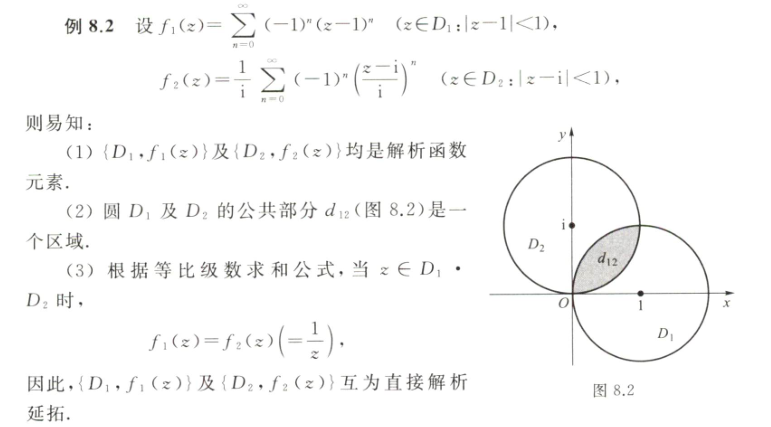
\includegraphics[width=\textwidth]{解析延拓-刷题-2025060923.png}
% \caption{}
\label{}
\end{figure}

\begin{figure}[H]
\centering
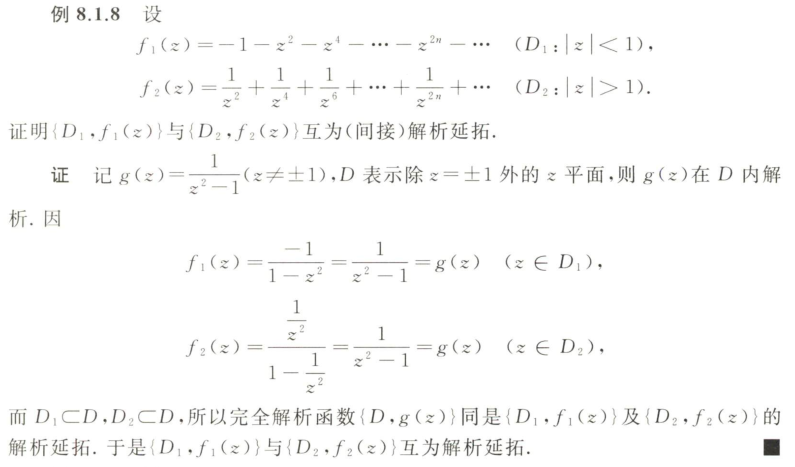
\includegraphics[width=\textwidth]{2-解析延拓-刷题-2025060923.png}
% \caption{}
\label{}
\end{figure}

\subsection{构造解析延拓链}

\begin{figure}[H]
\centering
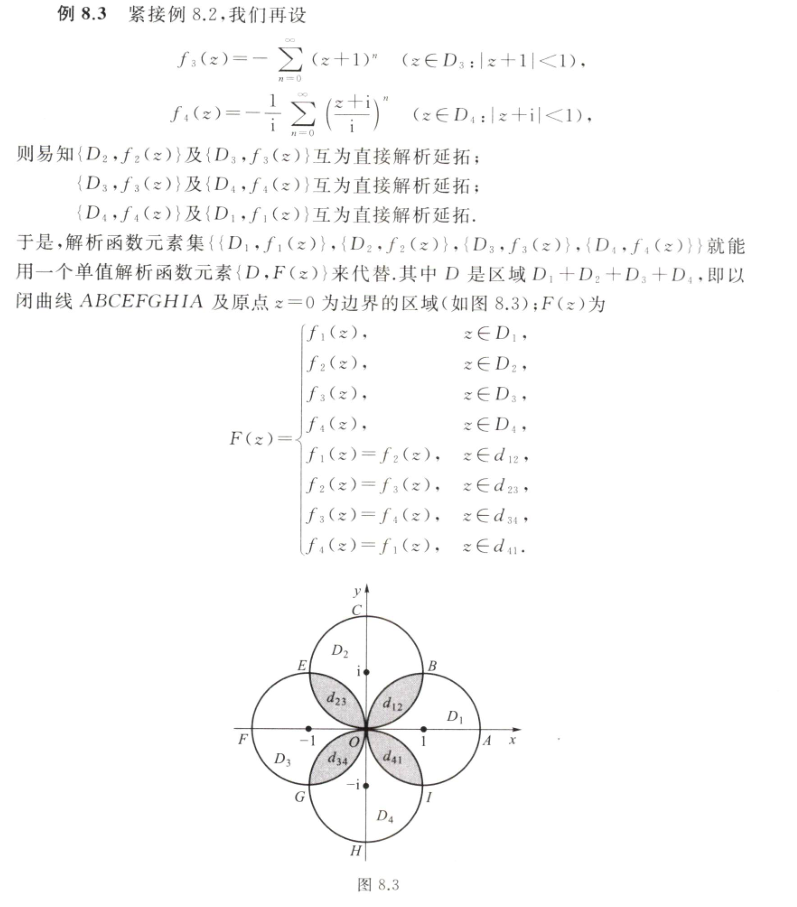
\includegraphics[width=\textwidth]{3-解析延拓-刷题-2025060923.png}
% \caption{}
\label{}
\end{figure}
\begin{figure}[H]
\centering
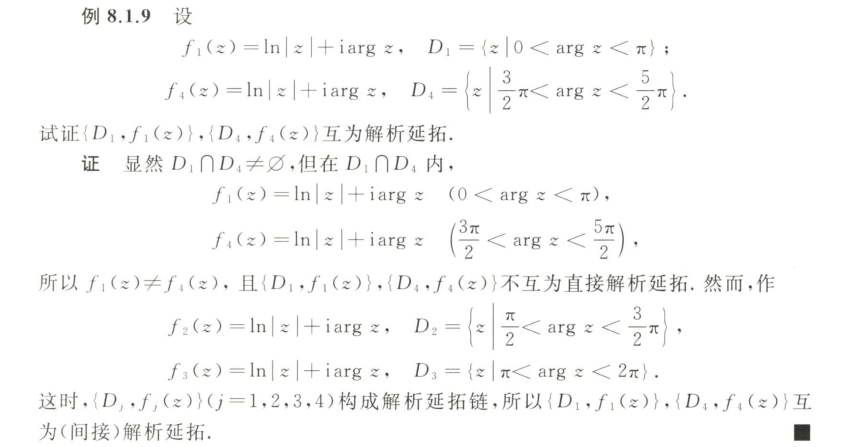
\includegraphics[width=\textwidth]{4-解析延拓-刷题-2025060923.png}
% \caption{}
\label{}
\end{figure}

\subsection{证明级数可延拓到整个复平面}

\begin{figure}[H]
\centering
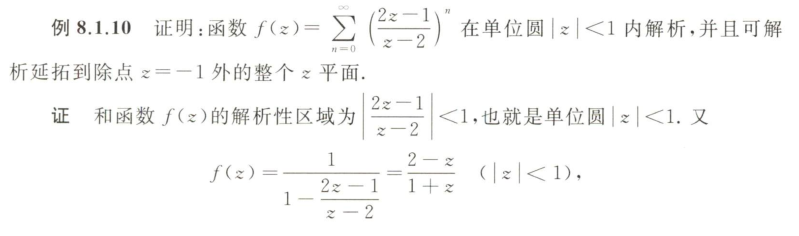
\includegraphics[width=\textwidth]{5-解析延拓-刷题-2025060923.png}
% \caption{}
\label{}
\end{figure}
\begin{figure}[H]
\centering

\includegraphics[width=\textwidth]{6-解析延拓-刷题-2025060923.png}
% \caption{}
\label{}
\end{figure}

\subsection{自然边界}

\begin{figure}[H]
\centering
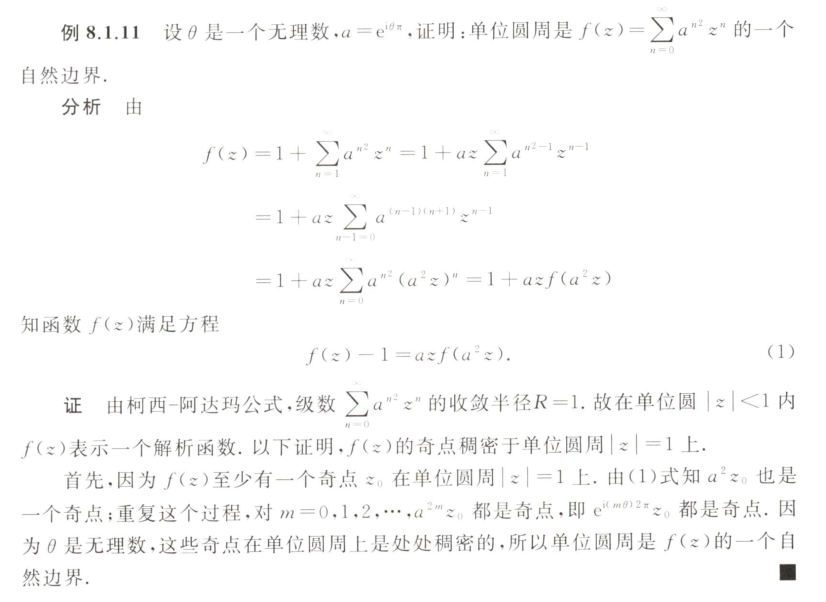
\includegraphics[width=\textwidth]{7-解析延拓-刷题-2025060923.png}
% \caption{}
\label{}
\end{figure}

\begin{figure}[H]
\centering
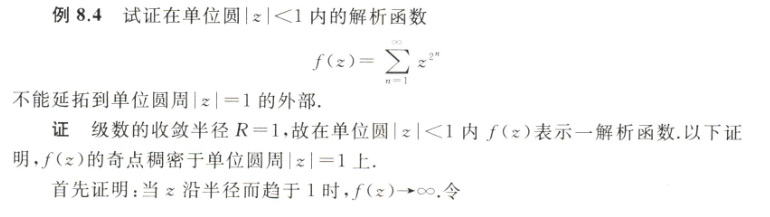
\includegraphics[width=\textwidth]{8-解析延拓-刷题-2025060923.png}
% \caption{}
\label{}
\end{figure}
\begin{figure}[H]
\centering
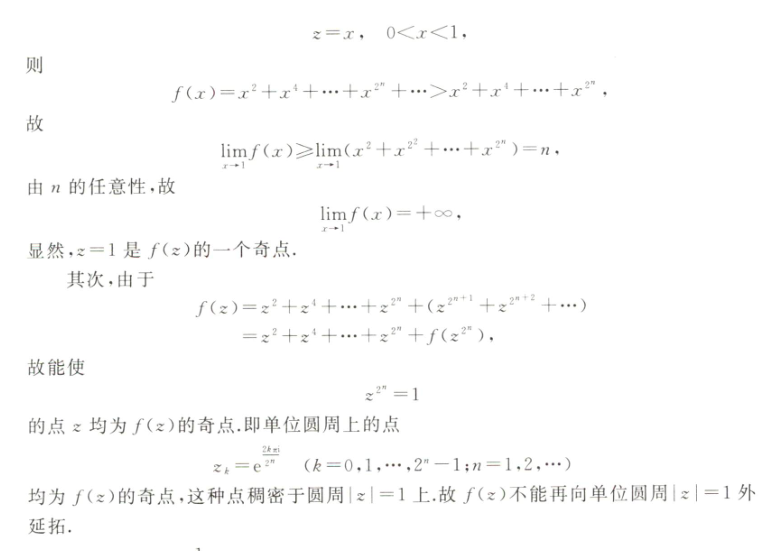
\includegraphics[width=\textwidth]{9-解析延拓-刷题-2025060923.png}
% \caption{}
\label{}
\end{figure}

\subsection{黎曼面的说明}

\begin{figure}[H]
\centering
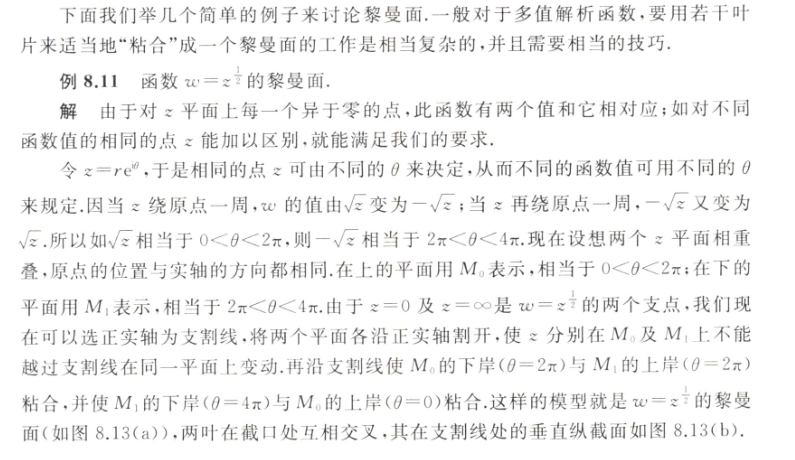
\includegraphics[width=\textwidth]{10-解析延拓-刷题-2025060923.png}
% \caption{}
\label{}
\end{figure}
\begin{figure}[H]
\centering
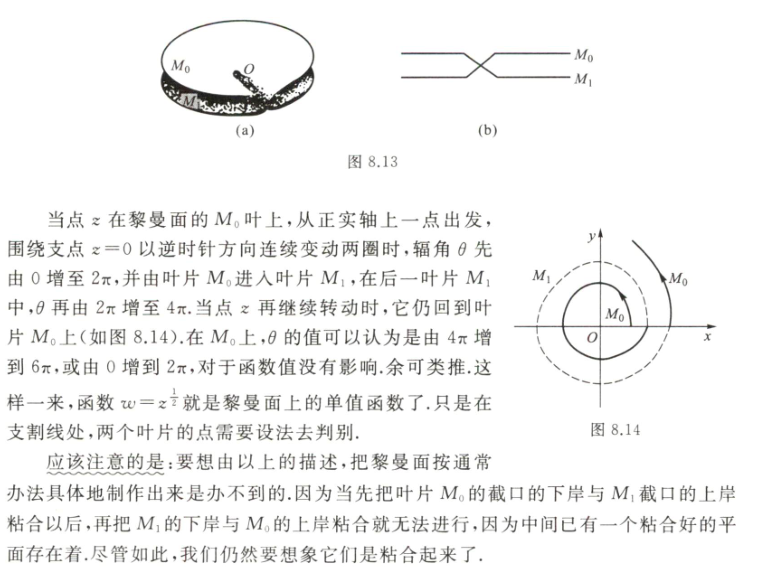
\includegraphics[width=\textwidth]{11-解析延拓-刷题-2025060923.png}
% \caption{}
\label{}
\end{figure}
\begin{figure}[H]
\centering
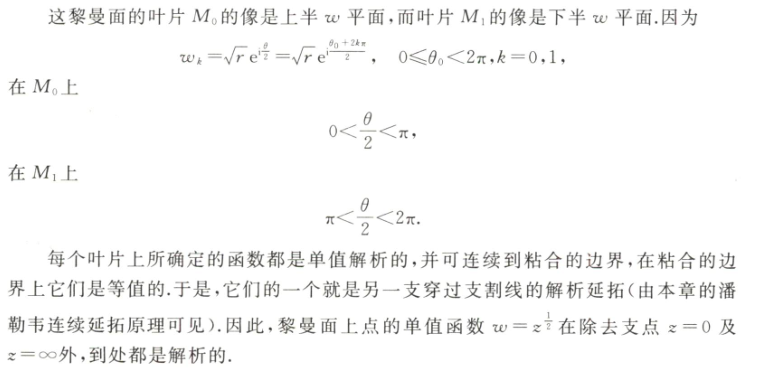
\includegraphics[width=\textwidth]{12-解析延拓-刷题-2025060923.png}
% \caption{}
\label{}
\end{figure}
\begin{figure}[H]
\centering
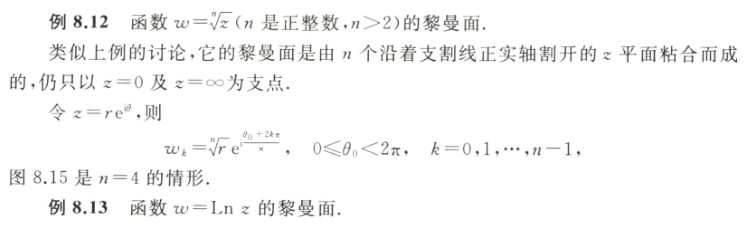
\includegraphics[width=\textwidth]{13-解析延拓-刷题-2025060923.png}
% \caption{}
\label{}
\end{figure}
\begin{figure}[H]
\centering
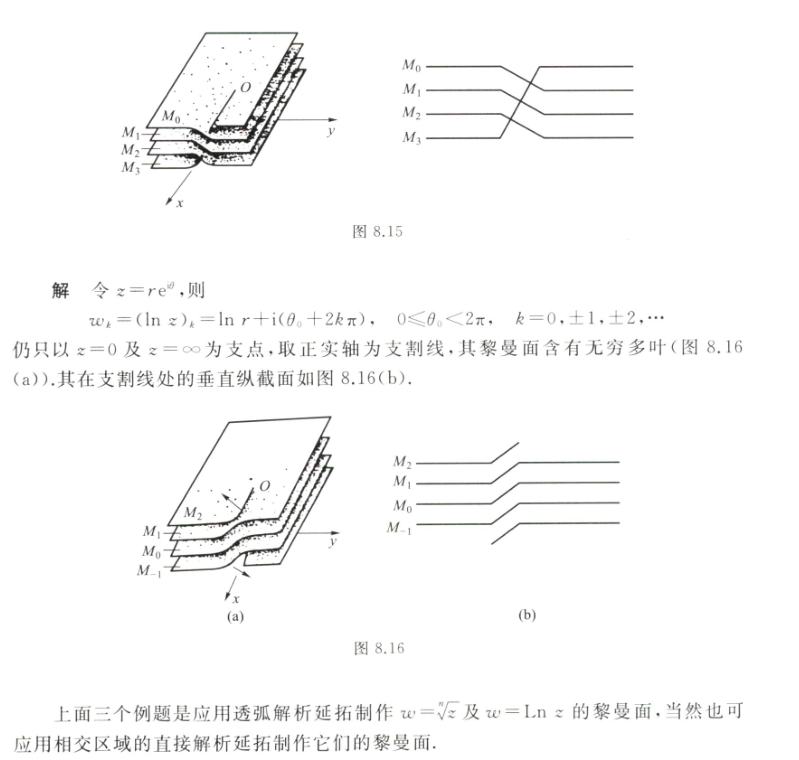
\includegraphics[width=\textwidth]{14-解析延拓-刷题-2025060923.png}
% \caption{}
\label{}
\end{figure}

\subsubsection{\texorpdfstring{$\sqrt[3]{ (z-a)(z-b) }$}{sqrt[3] (z-a)(z-b)} 的黎曼面}

\begin{figure}[H]
\centering
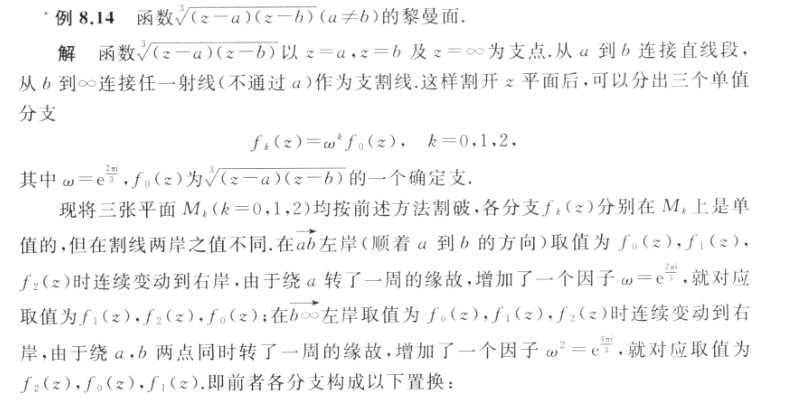
\includegraphics[width=\textwidth]{15-解析延拓-刷题-2025060923.png}
% \caption{}
\label{}
\end{figure}
\begin{figure}[H]
\centering
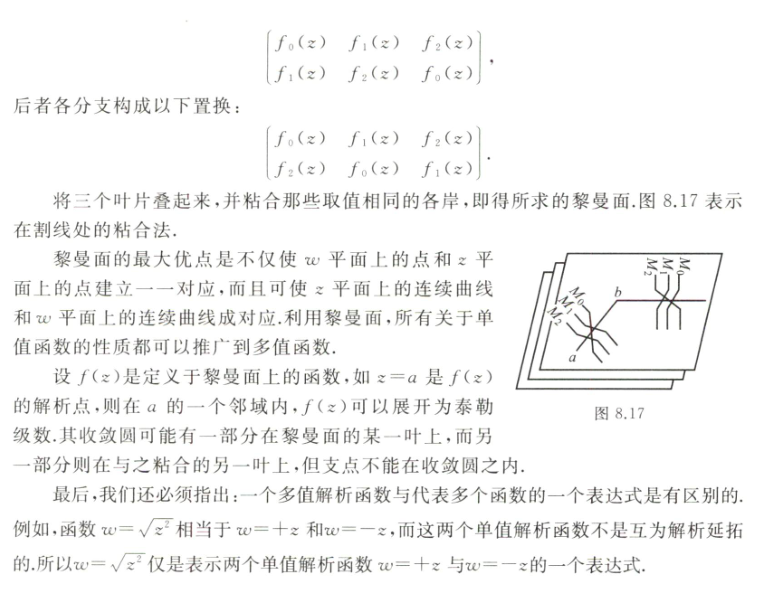
\includegraphics[width=\textwidth]{16-解析延拓-刷题-2025060923.png}
% \caption{}
\label{}
\end{figure}

\subsection{多角形区域共形映射}

\begin{figure}[H]
\centering
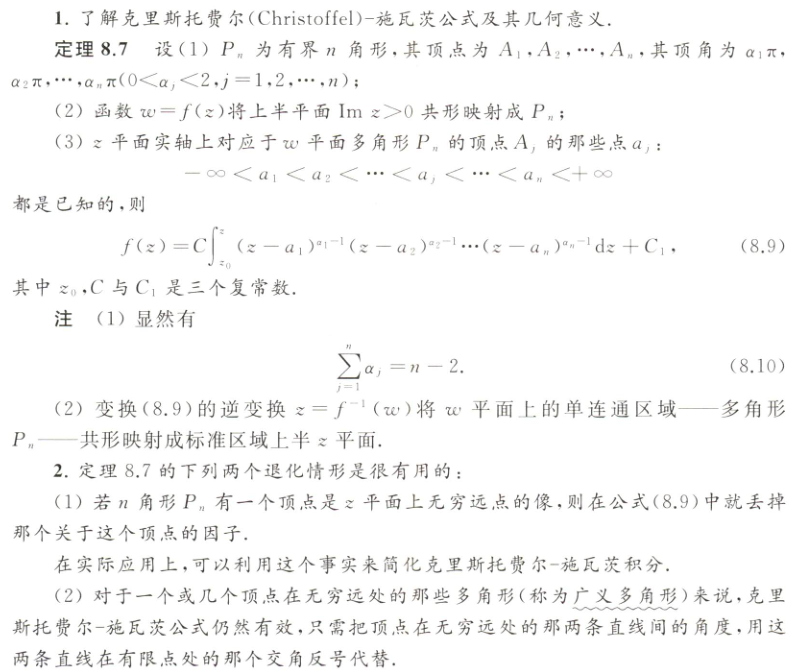
\includegraphics[width=\textwidth]{解析延拓-刷题-2025061000.png}
% \caption{}
\label{}
\end{figure}

\begin{remark}
由此可以看出,广义多角形实际上代表了扩充 $w$ 平面上许多特殊形状的单连通区域(边界不止一点)。而变换(8.9)的逆变换 $z=f^{-1}(w)$ 就能把这许多特殊形状的单连通区域共形映射成 (即"简化成")标准区域——上半 $z$ 平面.
\end{remark}
\subsubsection{广义多角形示例}

\begin{figure}[H]
\centering
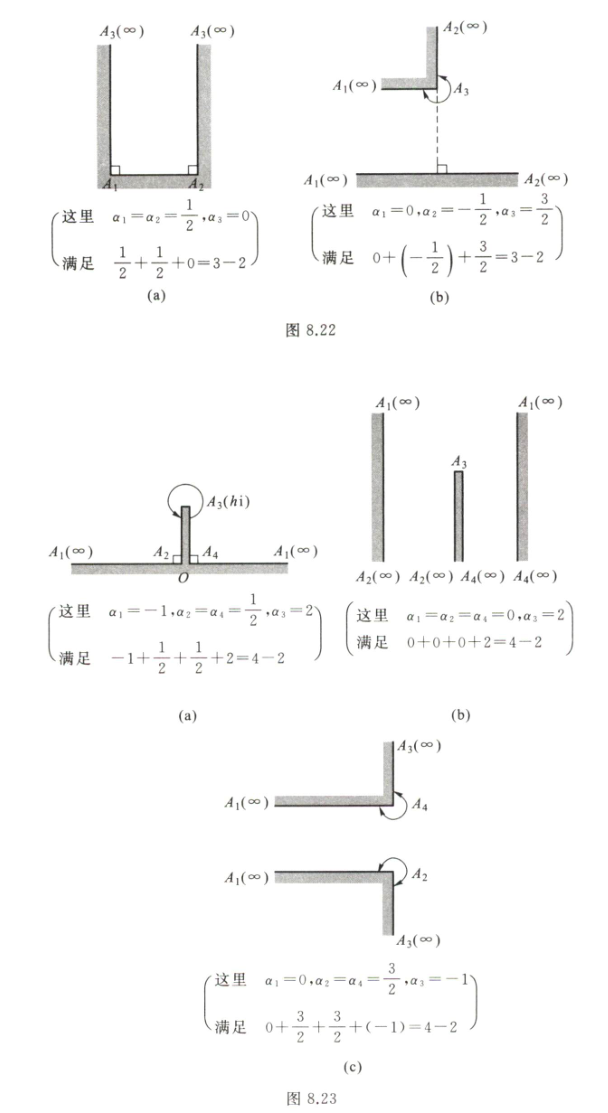
\includegraphics[width=\textwidth]{1-解析延拓-刷题-2025061000.png}
% \caption{}
\label{}
\end{figure}

对于 (a) 我们有

\begin{table}[h]
	\centering
	\begin{tabular}{|c|c|c|}
		\hline
		$A_j$ & $\alpha_{j}$ & $a_j$ \\
		\hline
		$-\frac{\pi}{2}$ & $\frac{1}{2}$ & -1 \\
		\hline
		$\frac{\pi}{2}$ & $\frac{1}{2}$ & 1 \\
		\hline
		$\infty$ & 0 & $\infty$ \\
		\hline
	\end{tabular}
\end{table}
于是根据 Schwarz-Christoffel 公式
\[
\begin{aligned}
w & =C\int_{0}^{z} (z+1)^{-\frac{1}{2}}(z-1)^{-\frac{1}{2}} \, \mathrm{d}z+C_1 \\
 & =C'\int_{0}^{z} \frac{1}{\sqrt{ 1-z^{2} }} \, \mathrm{d}z+C_1 \\
 & =C'\arcsin z+C_1
\end{aligned} 
\]
利用点 $a_1,a_2$ 与 $A_1,A_2$ 的对应关系,我们得到
\[
-\frac{\pi}{2}=-C'\cdot\frac{\pi}{2}+C_1,\quad \frac{\pi}{2}=C'\cdot\frac{\pi}{2}+C_1
\]
因此 $C_1=0,C'=1$. 故将上半 $z$ 平面 $\text{Im }z>0$,映射到半带形区域 $-\frac{\pi}{2}<\mathrm{Re }w<\frac{\pi}{2},\text{Im }w>0$ 的函数为
\[
w=\arcsin z
\]
取 $z=1$ 时, $w=\arcsin z=\frac{\pi}{2}$ 的那一支.

\begin{figure}[H]
\centering
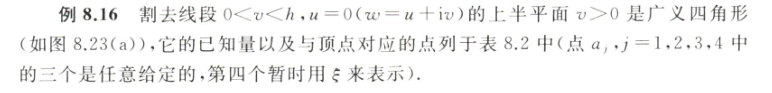
\includegraphics[width=\textwidth]{2-解析延拓-刷题-2025061000.png}
% \caption{}
\label{}
\end{figure}

\begin{table}[h]
	\centering
	\begin{tabular}{|c|c|c|}
		\hline
		$A_j$ & $\alpha _j$ & $a_{j}$ \\
		\hline
		$\infty$ & -1 & $\infty$ \\
		\hline
		0 & $\frac{1}{2}$ & -1 \\
		\hline
		$h \mathrm{i}$ & 2 & 0 \\
		\hline
		0 & $\frac{1}{2}$ & $\xi$ \\
		\hline
	\end{tabular}
\end{table}
\begin{figure}[H]
\centering
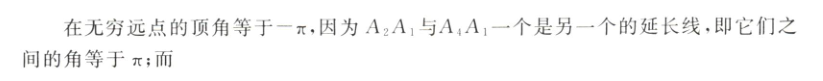
\includegraphics[width=\textwidth]{4-解析延拓-刷题-2025061000.png}
% \caption{}
\label{}
\end{figure}
\begin{figure}[H]
\centering
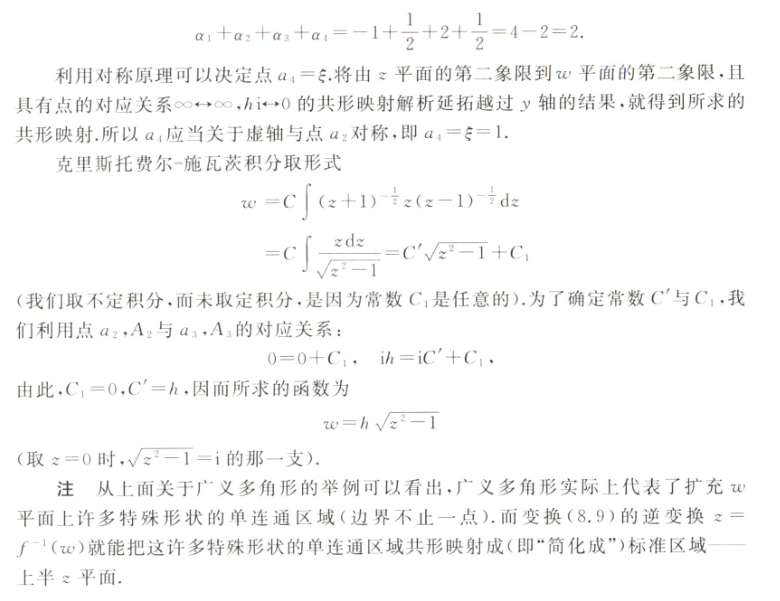
\includegraphics[width=\textwidth]{3-解析延拓-刷题-2025061000.png}
% \caption{}
\label{}
\end{figure}
